\documentclass[12pt]{article}

\usepackage{amsmath, amsthm, amssymb, amsfonts}
\usepackage{derivative, cancel, hyperref, bookmark}
\usepackage[english]{babel}
\usepackage[Rejne]{fncychap}
\usepackage[utf8]{inputenc}
\usepackage[T1]{fontenc}
\usepackage{mathpazo}
\usepackage{caption, subcaption}
\usepackage[dvipsnames]{xcolor}
\usepackage{tcolorbox, color, soul}
\usepackage[a4paper, portrait, margin=1.5cm]{geometry}
\tcbuselibrary{theorems, skins, breakable}
\hypersetup{colorlinks=true, linkcolor=blue, filecolor=magenta, urlcolor=cyan}

\begin{document}

\begin{titlepage}
	\newcommand{\HRule}{\rule{\linewidth}{0.5mm}}
	\center
	
	% Headings
	\textsc{\Huge Systems and Control Engineering}\\[1.5cm]	
	\textsc{\LARGE\bfseries SC649: Embedded Controls and Robotics}\\[1cm] % Major heading
	
	% Title
	\HRule\\[0.4cm]	
	{\huge\bfseries Assignment 2}\\[0.2cm] % Title of your document
	\HRule\\[1.5cm]
	
	% Author(s)
	\begin{minipage}{0.4\textwidth}
		\begin{flushleft}
			\large
			\textit{Team}\\
			\textsc{Pranav Gupta} (\texttt{22B2179})\\
			\textsc{Rohan Mekala} (\texttt{22B2106})\\
			\textsc{Sahil Sudhakar} (\texttt{210010055})\\
		\end{flushleft}
	\end{minipage}
	~
	\begin{minipage}{0.4\textwidth}
		\begin{flushright}
			\large
			\textit{Instructor}\\
			\textsc{Prof. Leena Vachhani}\\
            \href{mailto:leena.vachhani@iitb.ac.in}{leena.vachhani@iitb.ac.in}
		\end{flushright}
	\end{minipage}
	
	% Logo
	\vfill\vfill\vfill
	\includegraphics[width=0.4\textwidth]{/home/pranav/Documents/LaTeX/SysCon/logo.png}\\[1cm]
	
	% Date
	\vfill\vfill
	{\LARGE \today}
	\vfill
	
\end{titlepage}

\pagebreak
\tableofcontents

\section*{Work Distribution}
\begin{enumerate}
	\item \textbf{Pranav Gupta} (\texttt{22B2179}): Simulink model and stability analysis
	\item \textbf{Rohan Mekala} (\texttt{22B2106}): exponential velocity control strategy
	\item \textbf{Sahil Sudhakar} (\texttt{210010055}): ROS 1 Noetic - TurtleBot3 simulation
\end{enumerate}

\pagebreak

\section{Block Diagram Setup}
All the simulations in this assignment have been run with a fixed step size of \(50\,\mu\text{s}\) using \texttt{ode4} solver with a stop time of 10 seconds.

\begin{figure}[ht!]
	\centering
	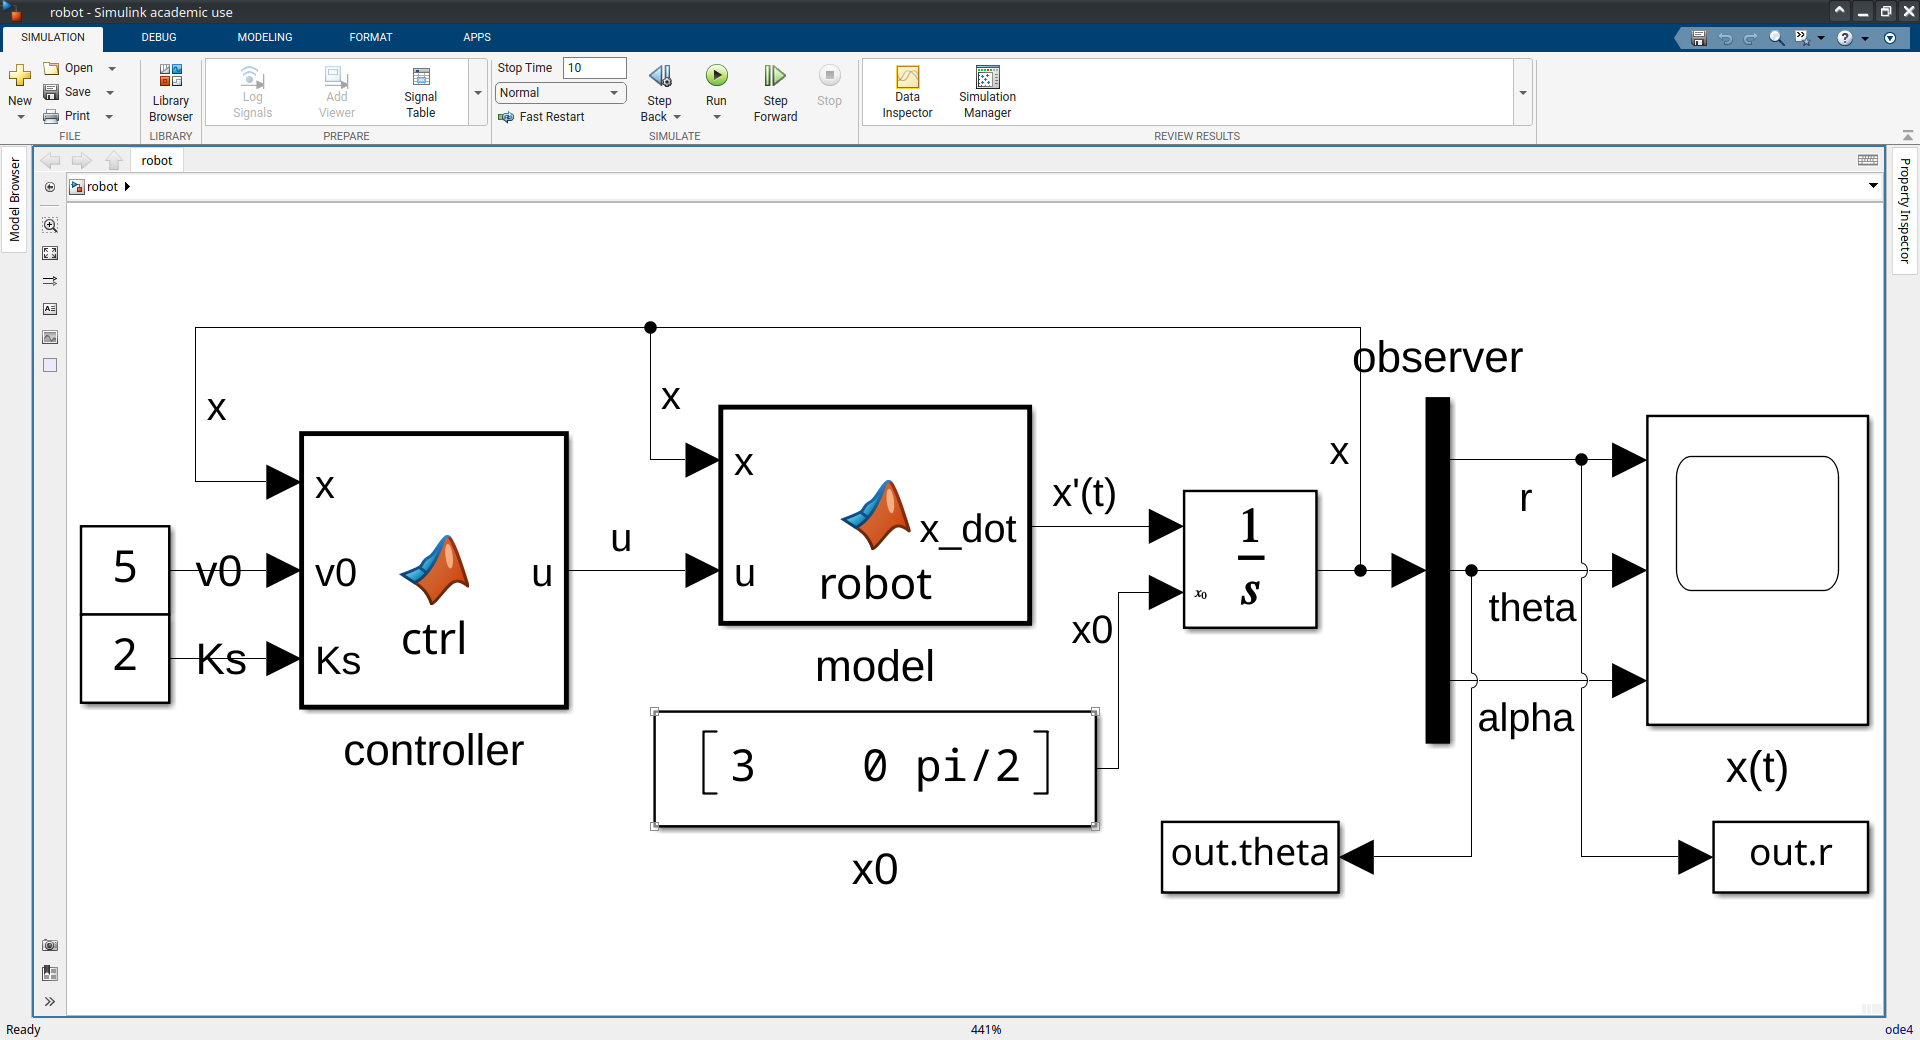
\includegraphics[width=0.6\linewidth]{images/simulink.png}
	\caption{screenshot of simulink model used to simulate and conduct analysis}
\end{figure}

\section{Plant and Controller}

The plant of the kinematics of the robot model is:
\[\begin{aligned}
	\dot{r} &= v\cos(\alpha-\theta) \\
	\dot{\theta} &= \frac{v}{r}\sin(\alpha-\theta)\\
	\dot{\alpha} &= \omega
\end{aligned}\]
The control law that we have used is as follows:

\[\begin{aligned}
	v &= v_0 \\
	\omega &= -K_s \cdot \text{sgn}(\alpha - \theta - \pi)
\end{aligned}\]

\section{Implementation}
We have successfully implemented the steering control as the system response is converging and the robot settles down at the home position.

\begin{figure}[h]
    \centering
    \begin{subfigure}{.32\textwidth}
        \centering
        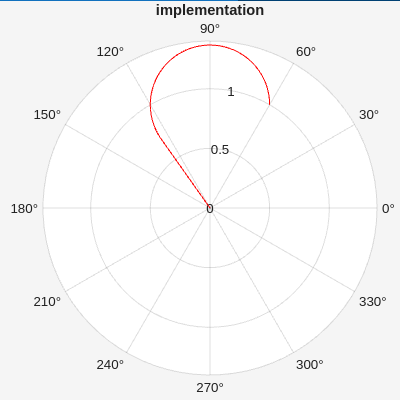
\includegraphics[width=0.9\linewidth]{images/implementplot.png}
    \end{subfigure}
    \begin{subfigure}{.65\textwidth}
        \centering
        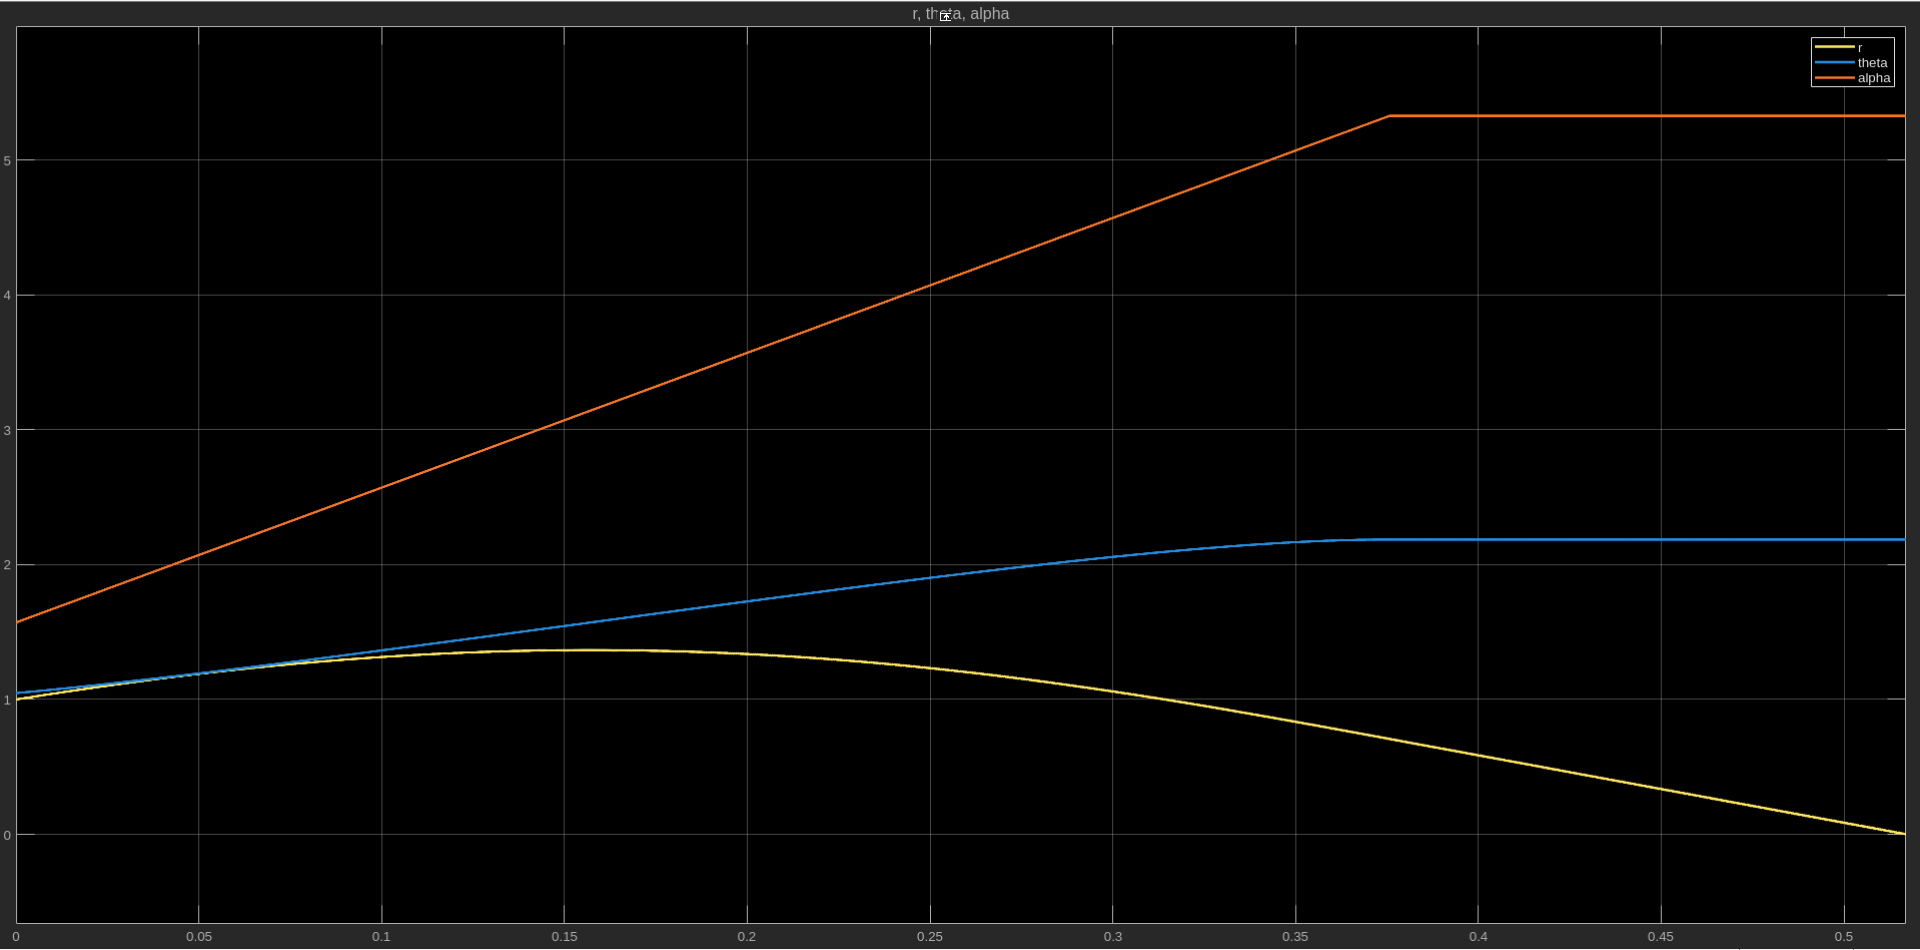
\includegraphics[width=0.9\linewidth]{images/implementscope.png}
    \end{subfigure}
    \caption{system response for initial conditions \(\{R, \theta, \alpha\} = \{1, \frac{\pi}{3}, \frac{\pi}{2}\}\)}
\end{figure}

\pagebreak
\section{Response for Different Initial Positions in Each Quadrant:}

\begin{figure}[h]
    \centering
    \begin{subfigure}{.48\textwidth}
        \centering
        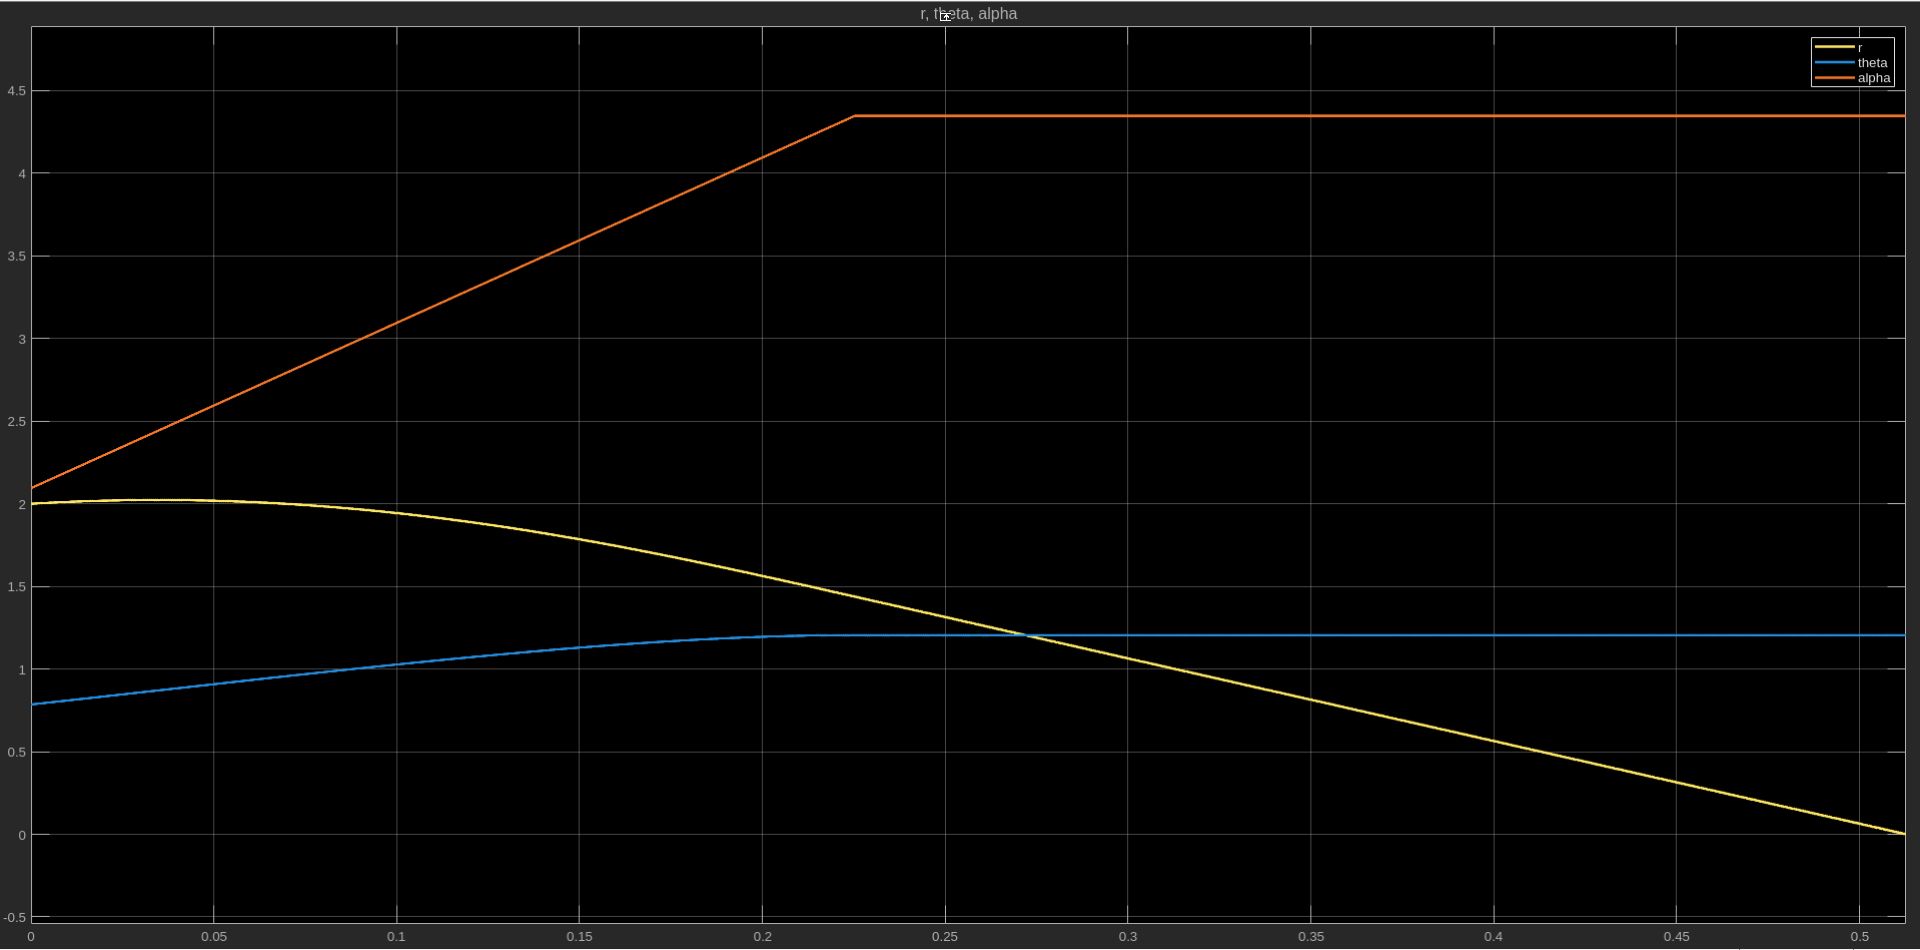
\includegraphics[width=0.9\linewidth]{images/Q1.png}
		\caption{\(\{R, \theta, \alpha\} = \left\{2, \frac{\pi}{4}, \frac{2\pi}{3}\right\}\)}
    \end{subfigure}
    \begin{subfigure}{.48\textwidth}
        \centering
        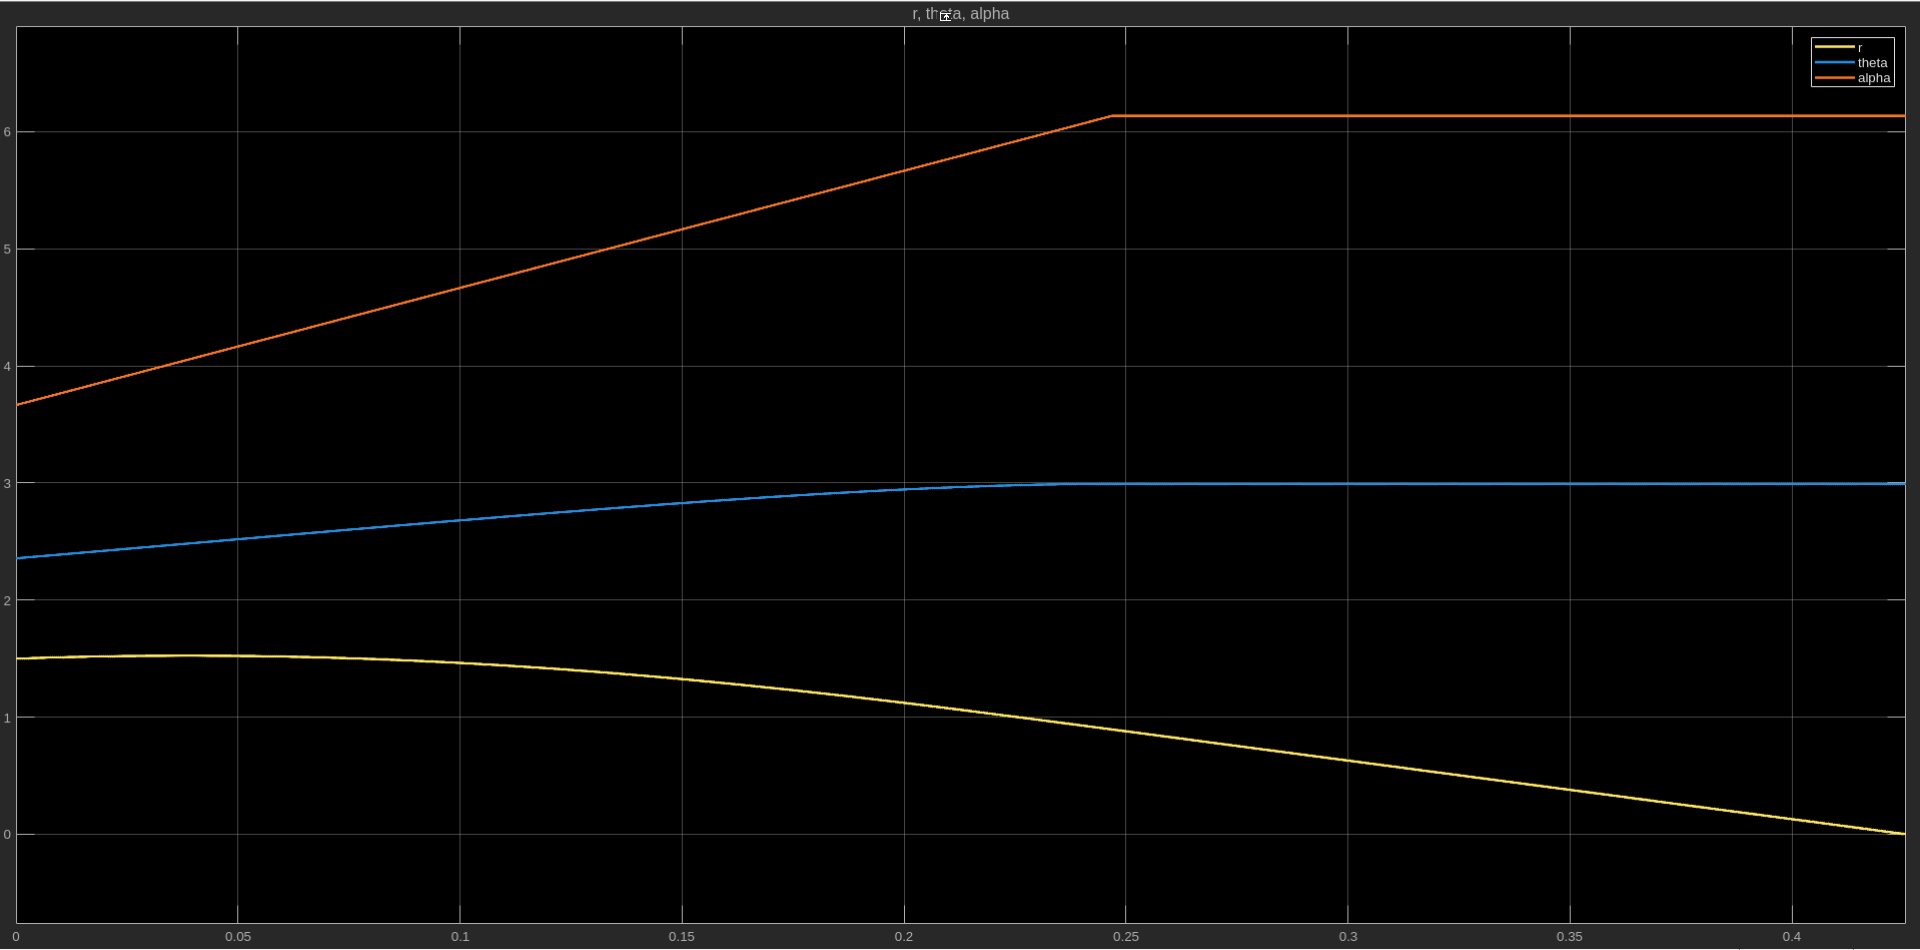
\includegraphics[width=0.9\linewidth]{images/Q2.png}
		\caption{\(\{R, \theta, \alpha\} = \left\{1.5, \frac{3\pi}{4}, \frac{7\pi}{6}\right\}\)}
    \end{subfigure}
	\begin{subfigure}{.48\textwidth}
        \centering
        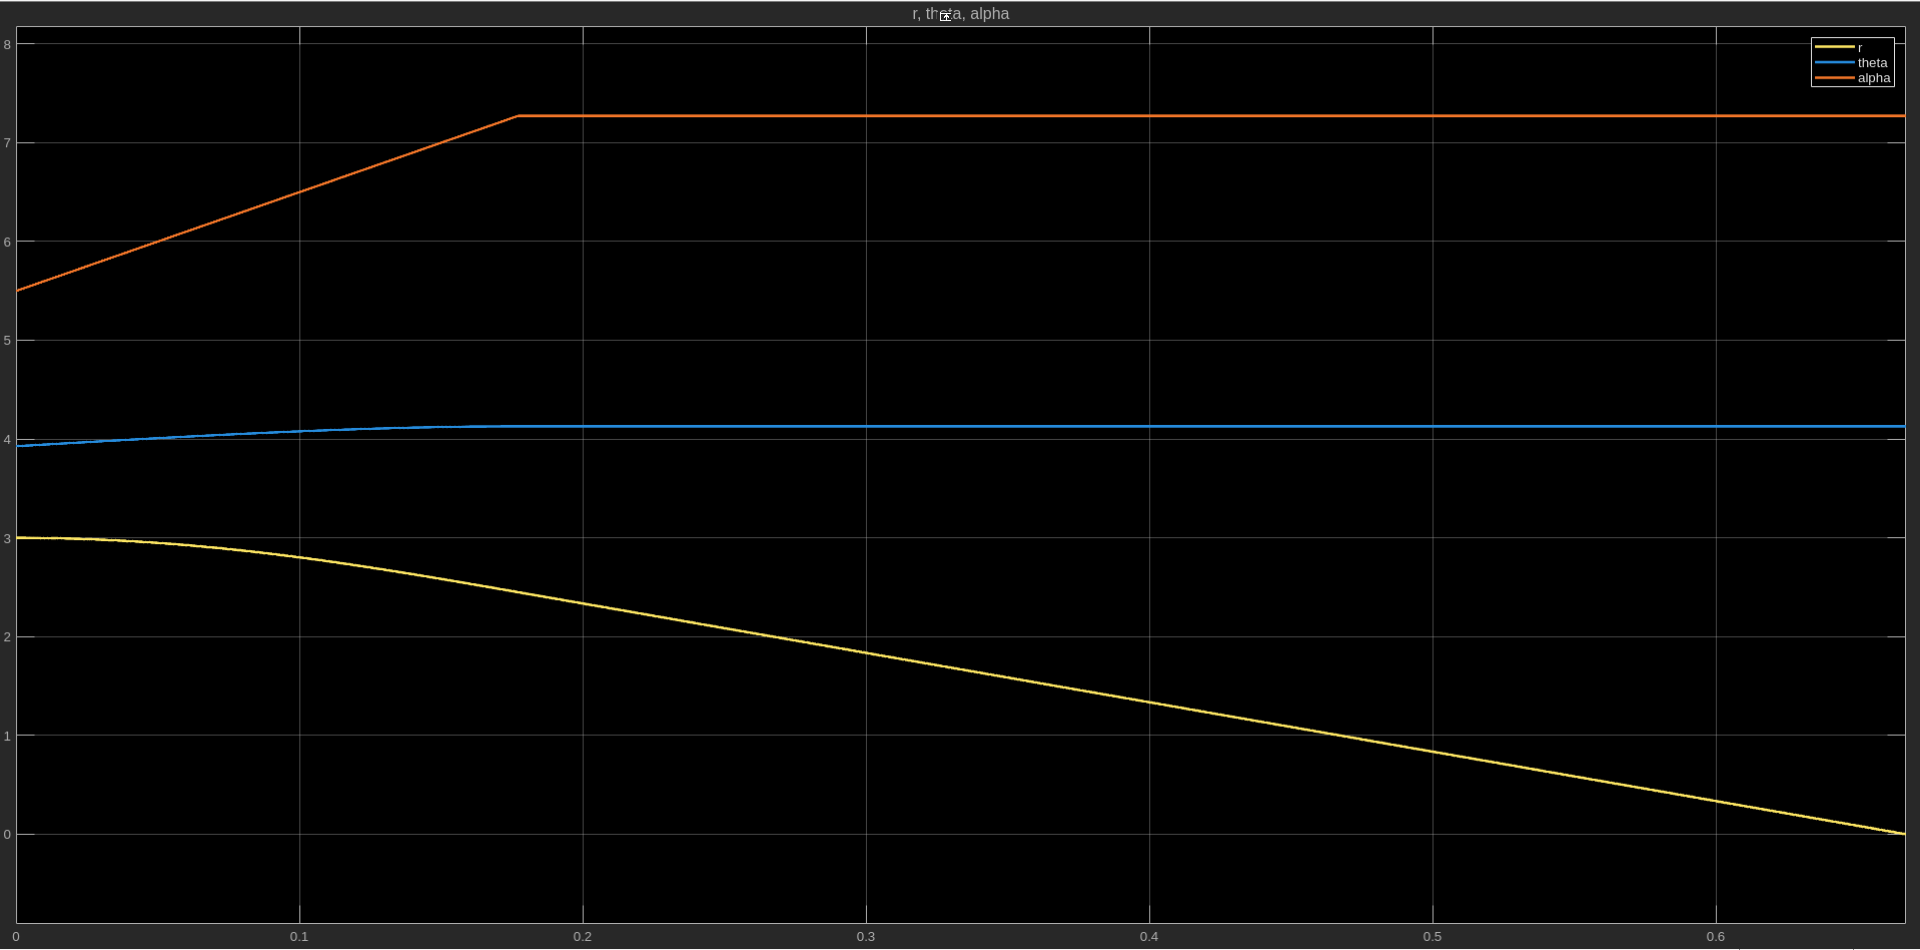
\includegraphics[width=0.9\linewidth]{images/Q3.png}
		\caption{\(\{R, \theta, \alpha\} = \left\{3, \frac{5\pi}{4}, \frac{7\pi}{4}\right\}\)}
    \end{subfigure}
    \begin{subfigure}{.48\textwidth}
        \centering
        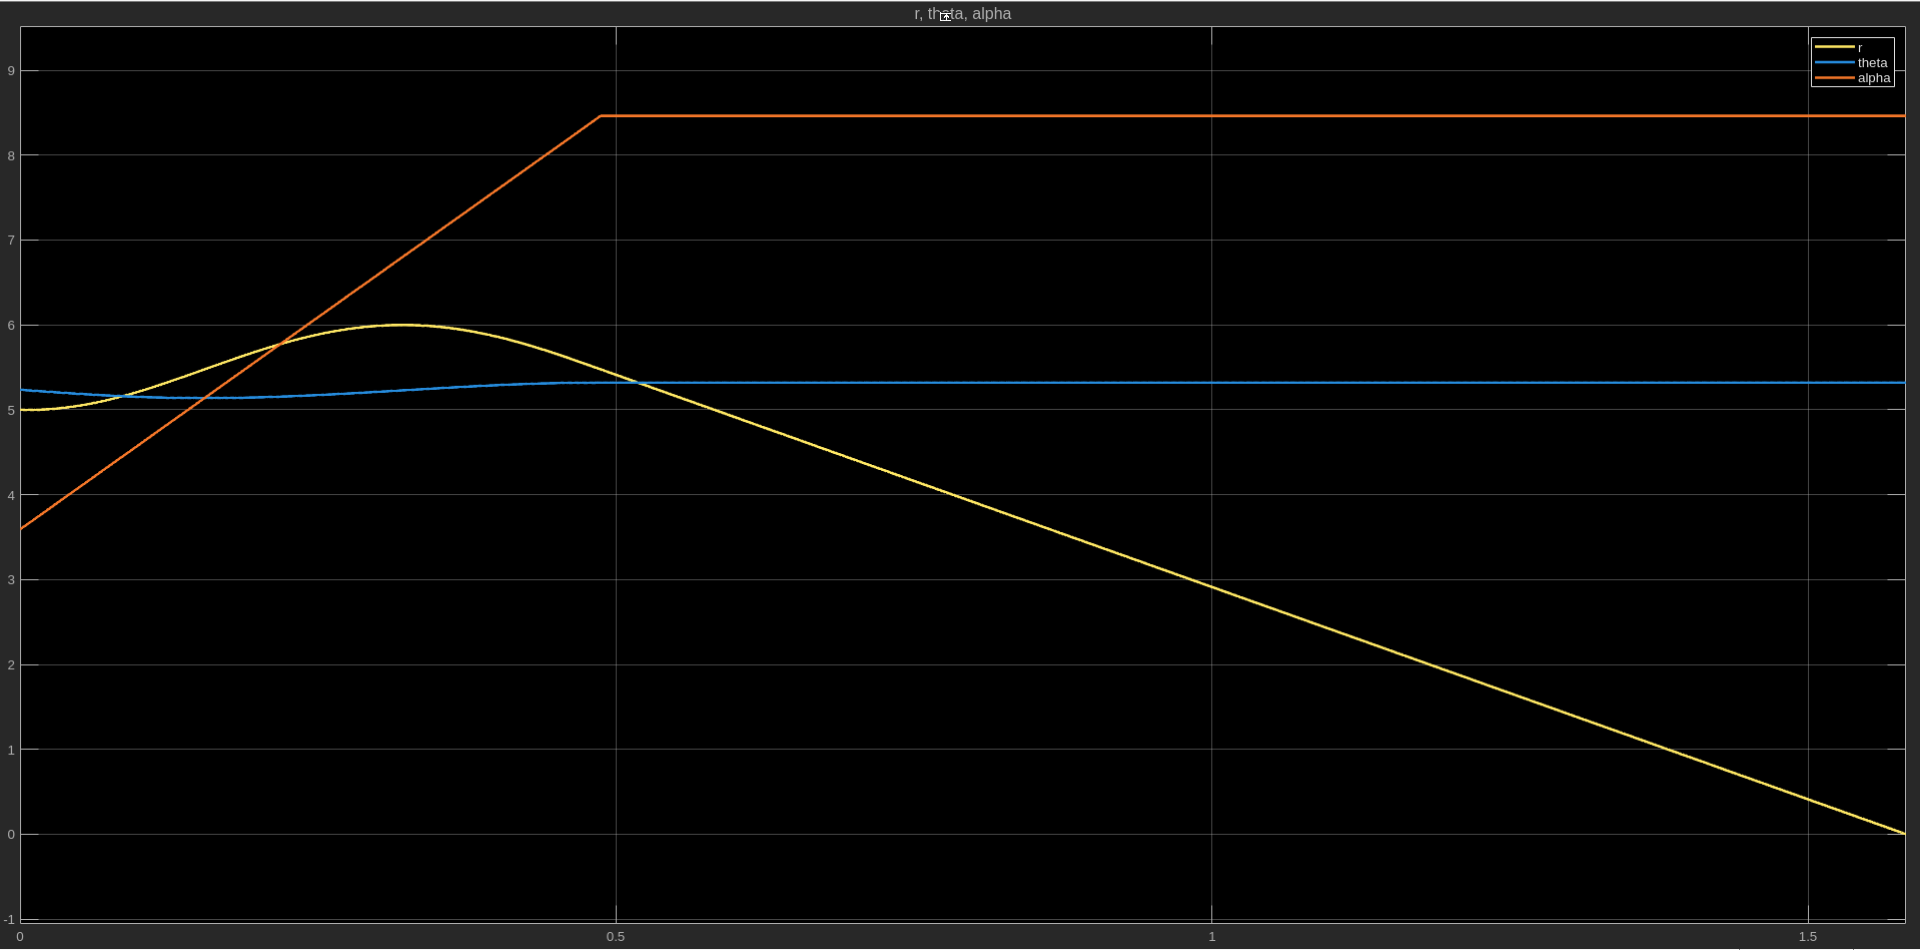
\includegraphics[width=0.9\linewidth]{images/Q4.png}
		\caption{\(\{R, \theta, \alpha\} = \left\{5, \frac{5\pi}{3}, \frac{8\pi}{7}\right\}\)}
    \end{subfigure}
    \caption{system response for initial conditions}
\end{figure}

\begin{figure}[ht!]
	\centering
	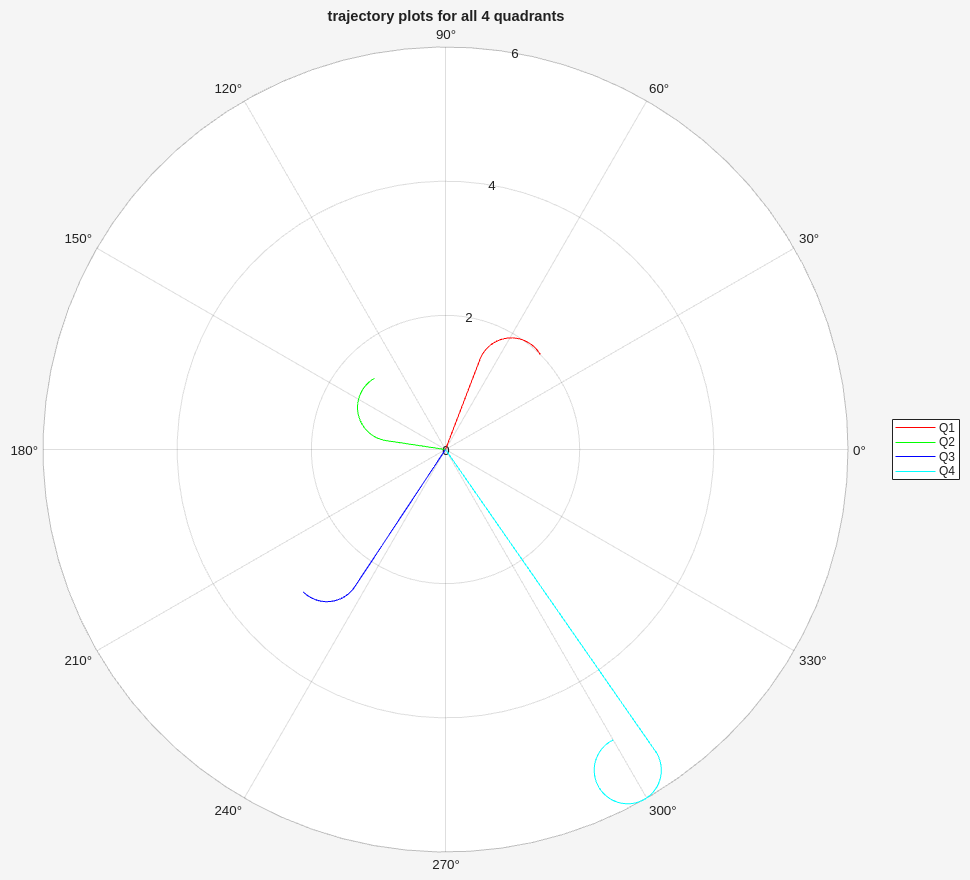
\includegraphics[width=0.75\linewidth]{images/quadrants.png}
	\caption{trajectories for all for quadrant initial conditions}
\end{figure}


\section{Response for Different Control Gains}
The initial conditions for this section are: \(\{R, \theta, \alpha\} = \left\{6, \frac{\pi}{3}, \frac{\pi}{4}\right\}\) and \(v_0 = 5, r_0 = 0.1\)
\begin{figure}[h]
    \centering
    \begin{subfigure}{.48\textwidth}
        \centering
        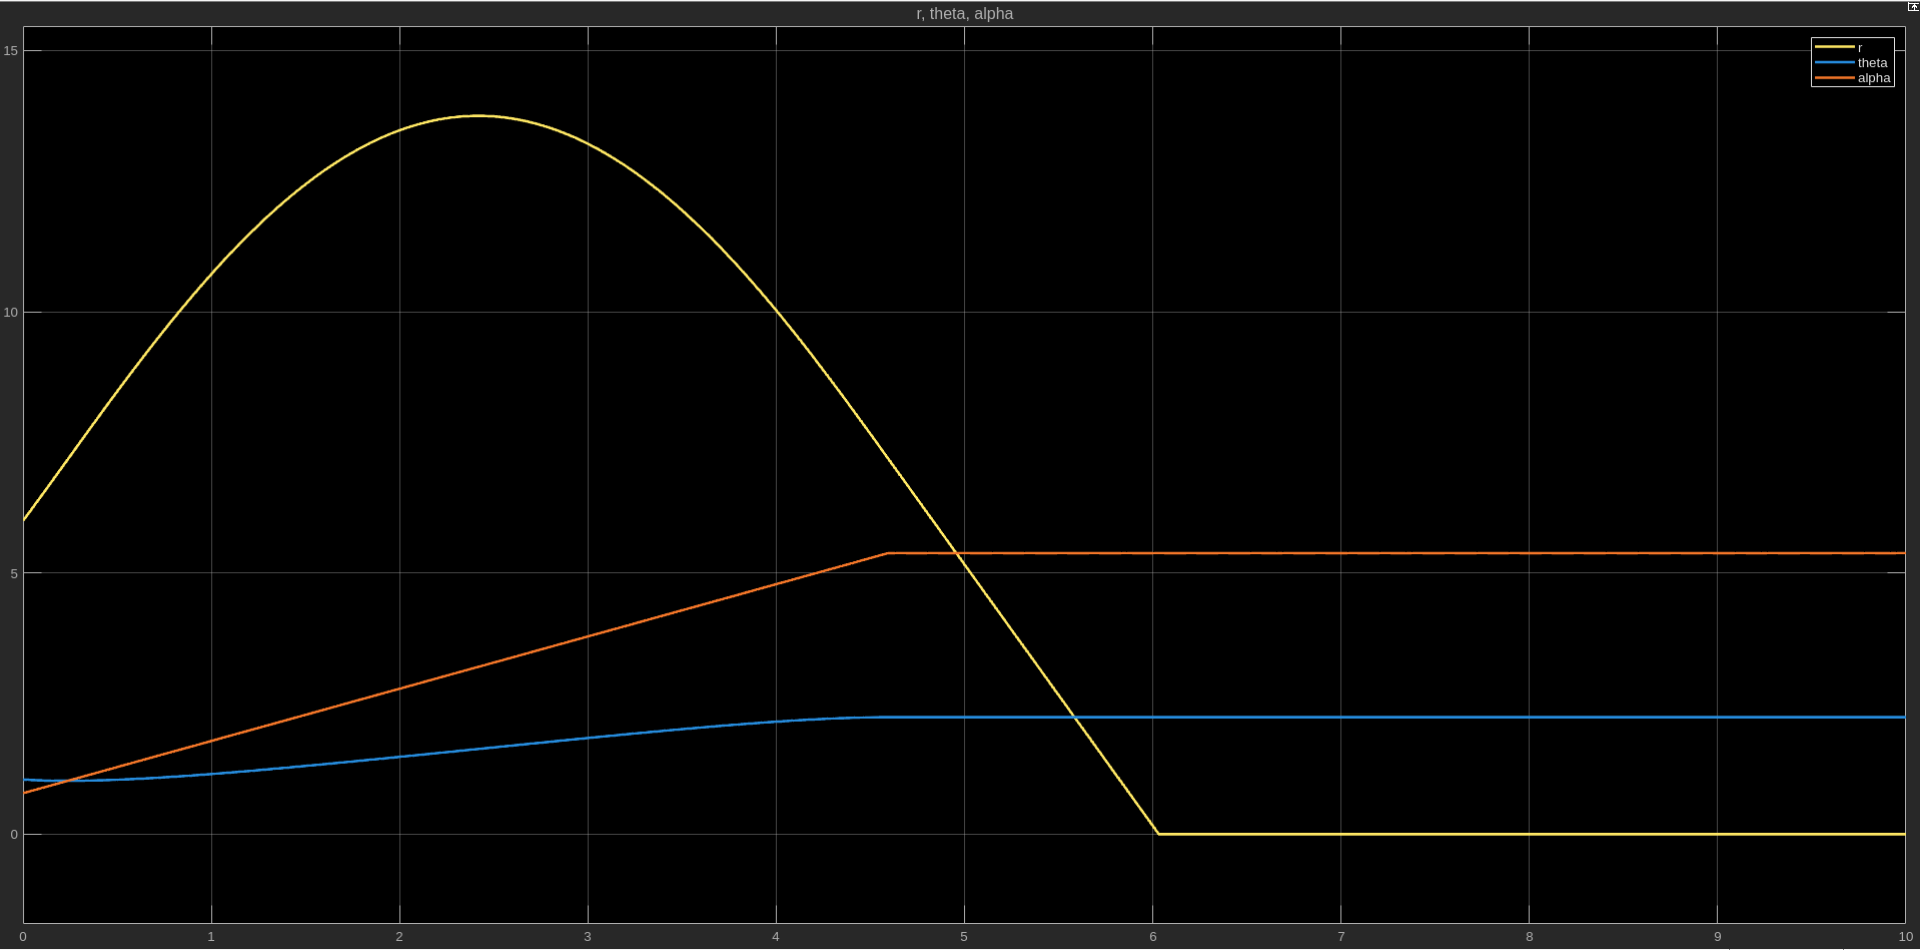
\includegraphics[width=0.9\linewidth]{images/K1.png}
		\caption{\(K_s=1\implies t_s=6.032\)}
    \end{subfigure}
    \begin{subfigure}{.48\textwidth}
        \centering
        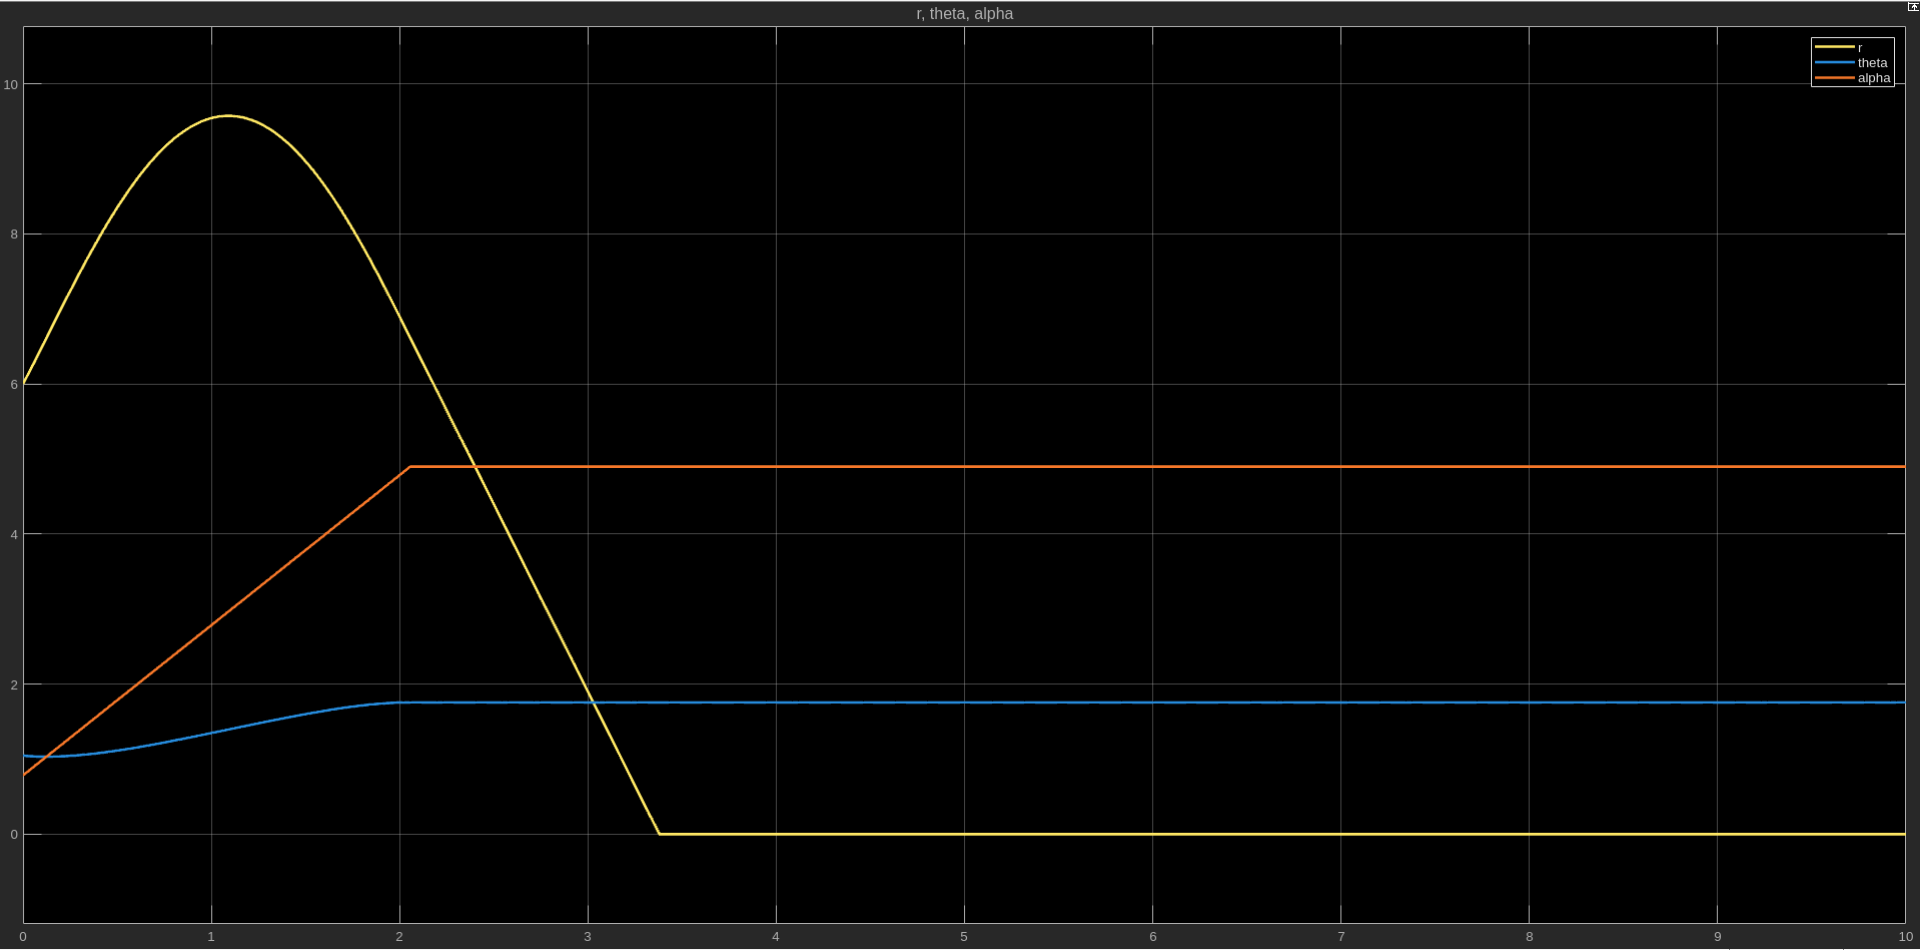
\includegraphics[width=0.9\linewidth]{images/K2.png}
		\caption{\(K_s=2\implies t_s=3.380\)}
    \end{subfigure}
	\begin{subfigure}{.48\textwidth}
        \centering
        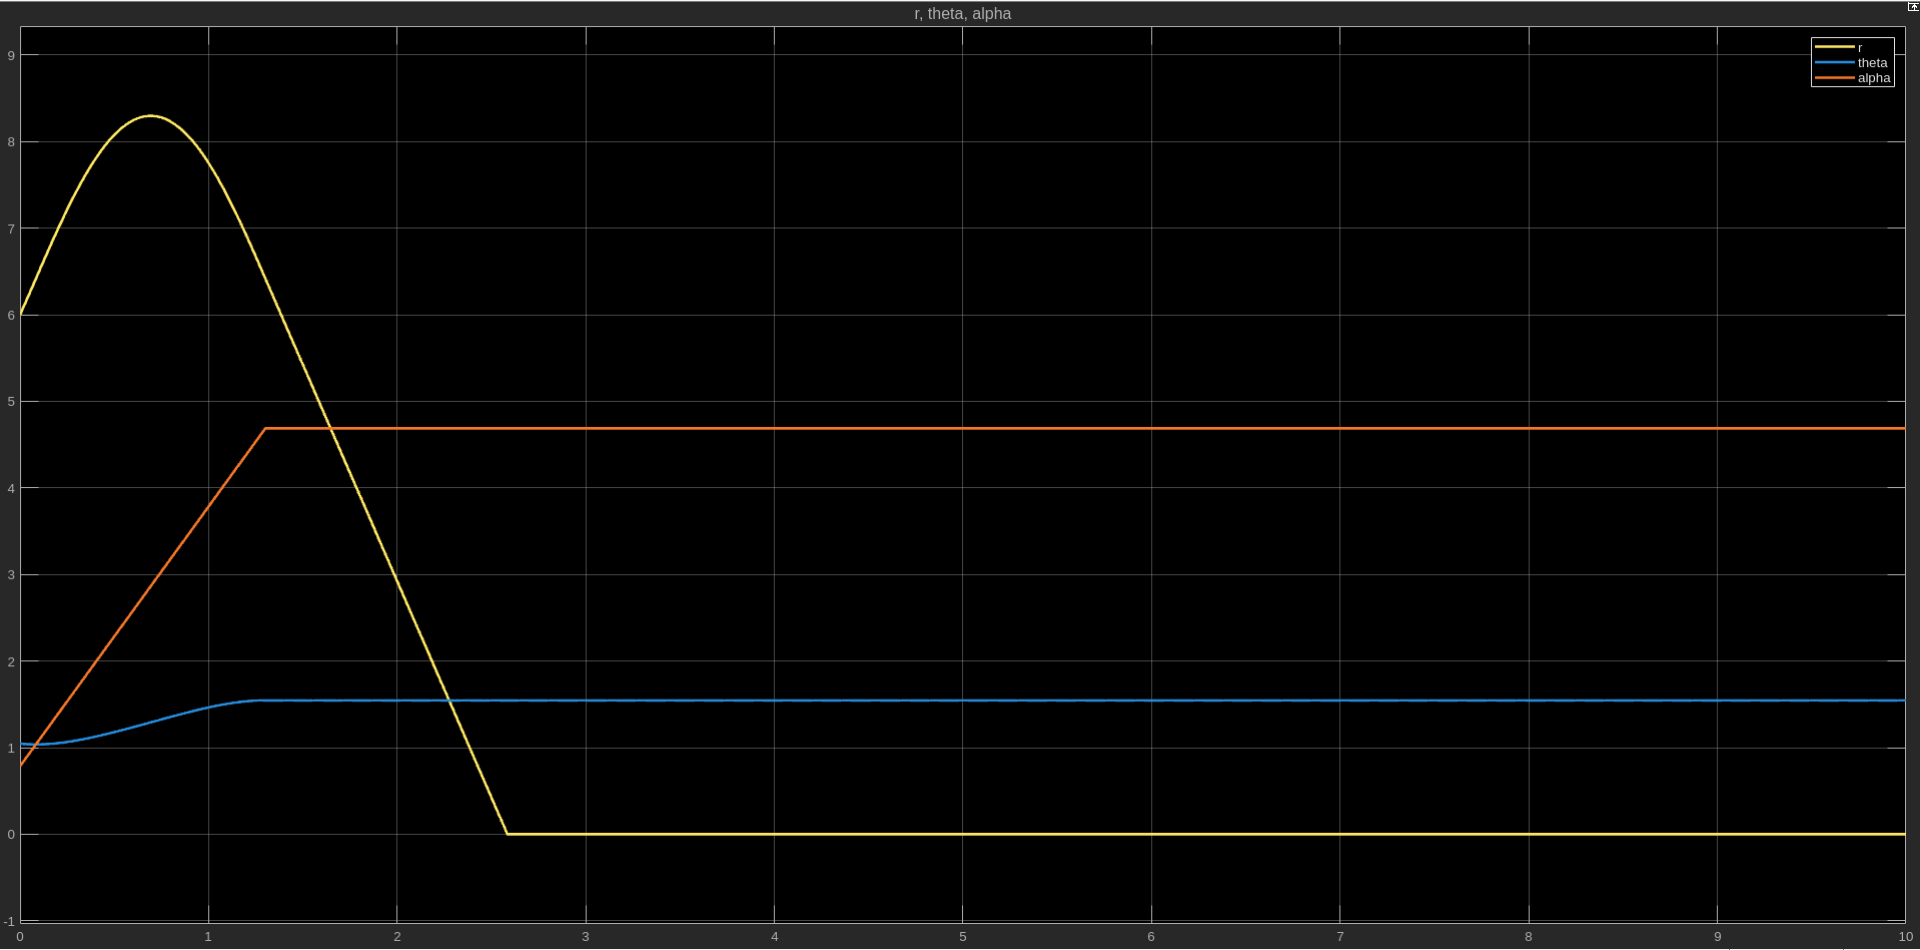
\includegraphics[width=0.9\linewidth]{images/K3.png}
		\caption{\(K_s=3\implies t_s=2.584\)}
    \end{subfigure}
    \begin{subfigure}{.48\textwidth}
        \centering
        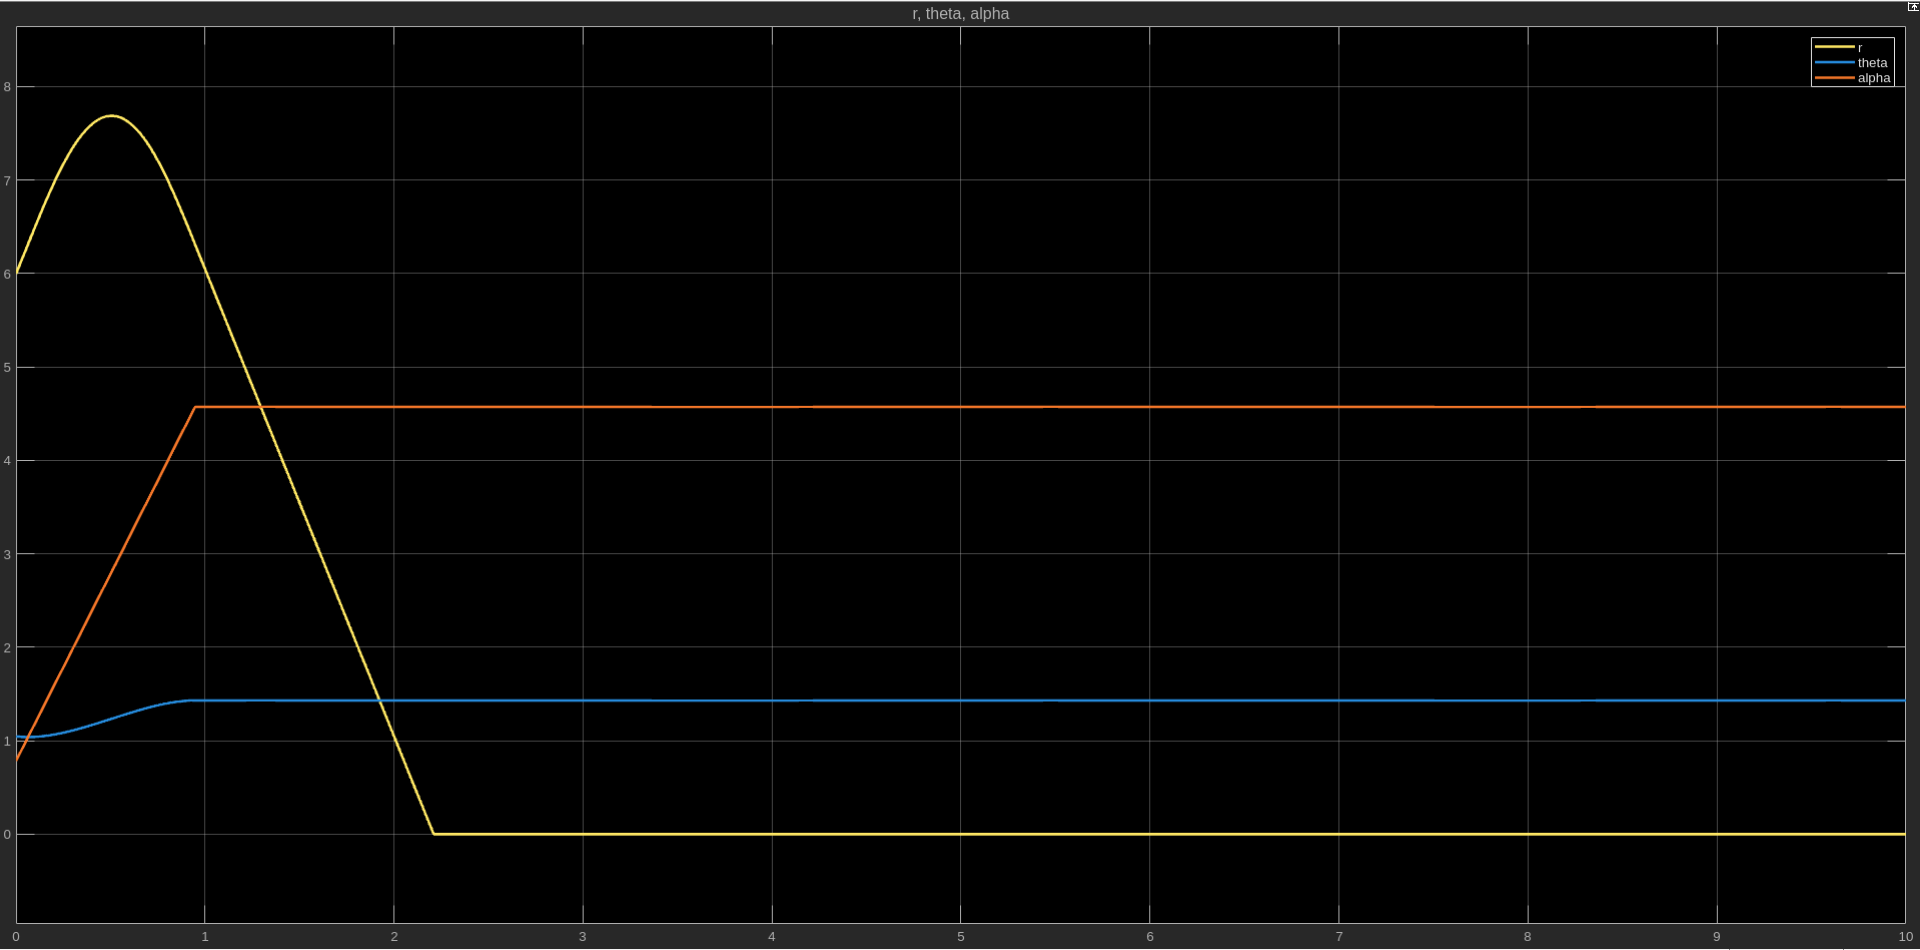
\includegraphics[width=0.9\linewidth]{images/K4.png}
		\caption{\(K_s=4\implies t_s=2.210\)}
    \end{subfigure}
	\begin{subfigure}{.48\textwidth}
        \centering
        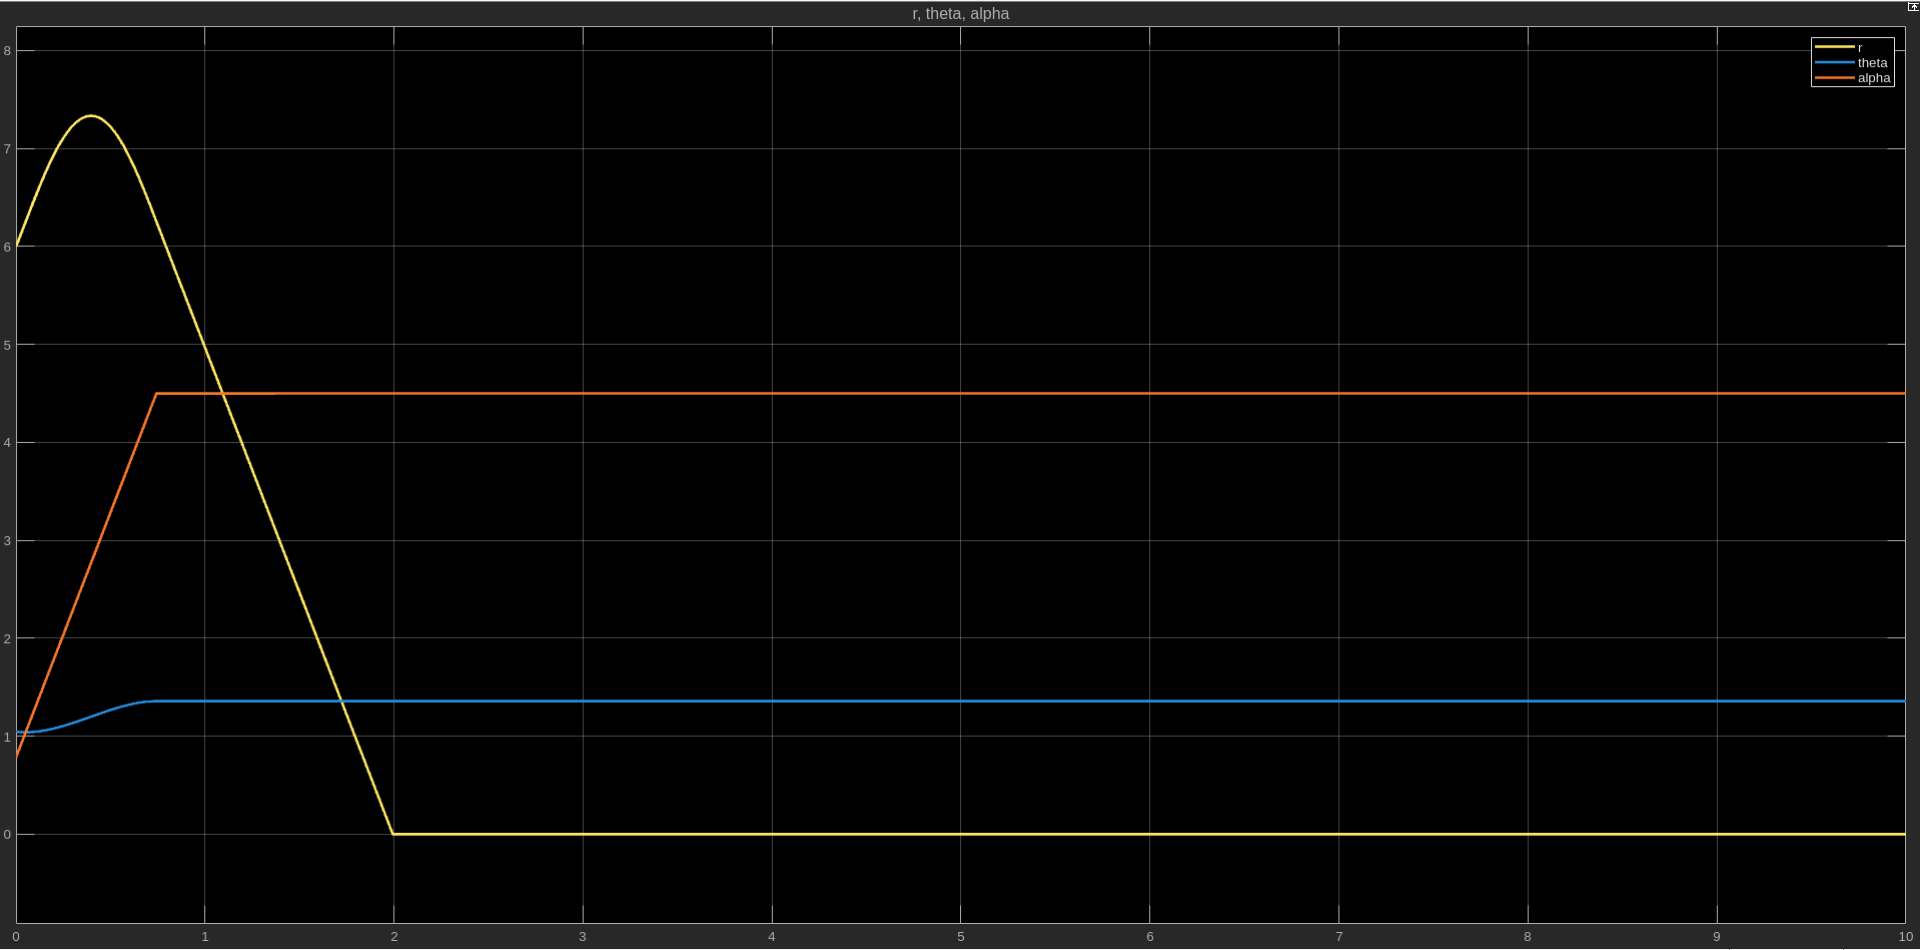
\includegraphics[width=0.9\linewidth]{images/K5.png}
		\caption{\(K_s=5\implies t_s=1.994\)}
    \end{subfigure}
    \caption{system response for \(K\in\{1,2,3,4,5\}\), robot being forcefully stopped when \(r\)}
\end{figure}

\begin{figure}[ht!]
	\centering
	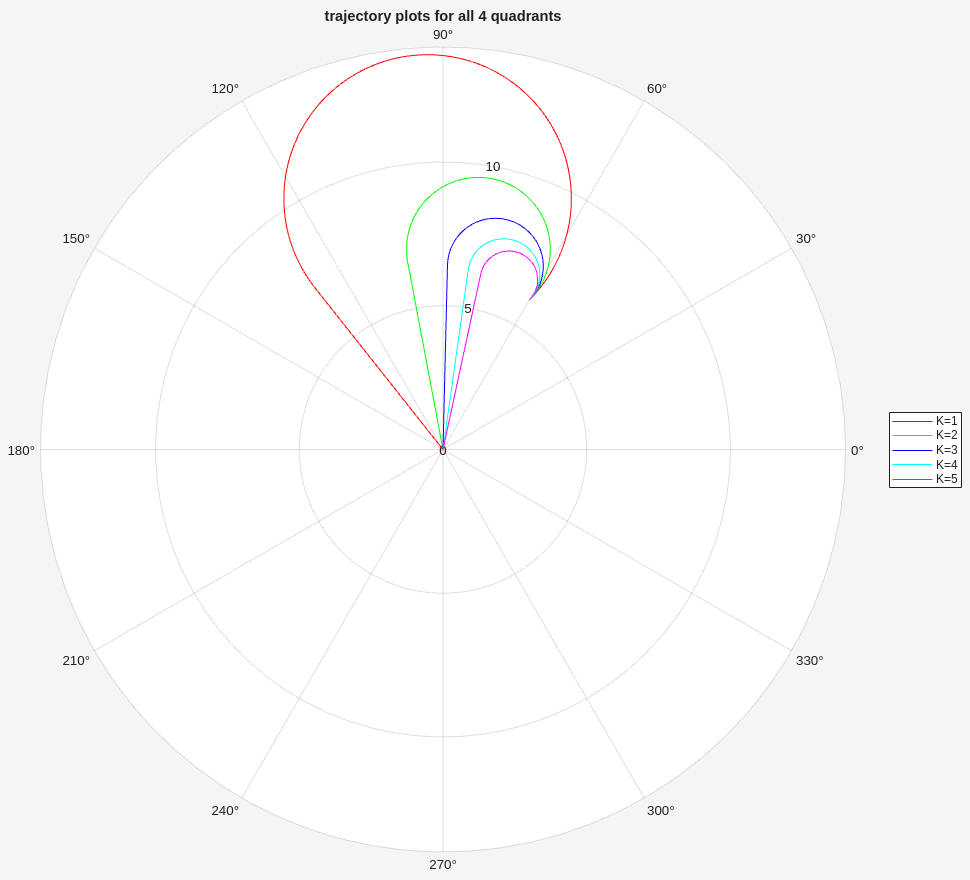
\includegraphics[width=0.5\linewidth]{images/K.png}
	\caption{trajectories for all for quadrant initial conditions}
\end{figure}

Increasing \(K_s\) decreases the settling time \(t_s\) and also decreases the maximum overshoot. Physically, this means the robot's maneuver towards the home position is tighter because \(\|\omega\|=K_s\), consequently dropping the settling time. One can also however notice that increasing \(K_s\) corresponds to installing a more powerful motor for the steering control, but at marginal returns on settling time for higher values of \(K_s\).

\section{Comments on Stability}

We were unable to identify any inital conditions for which the controller is unstable in the sense of divergence. However, we were able to identify a class of initial conditions for which the controller is marginally unstable in the sense of getting stuck in a loop without converging to the home position, where if the initial relative heading of the robot (\(\alpha_0-\theta_0\)) is such that the control law doesn't effectively reduce the angle error between the robot's current heading and the target heading (home position), the robot could end up in a loop where it perpetually adjusts its heading in a circular manner without ever reducing the radial distance \(R\) to the home position.

One such trivial case is when the initial relative heading \(\alpha_0-\theta_0=\frac{\pi}{2}\) and the initial radial distance \(\displaystyle r_0=\frac{v_0}{K_s}\) for which robot forever revolves about the origin in a fixed circle of radius \(r_0\).

\begin{figure}[ht!]
    \centering
    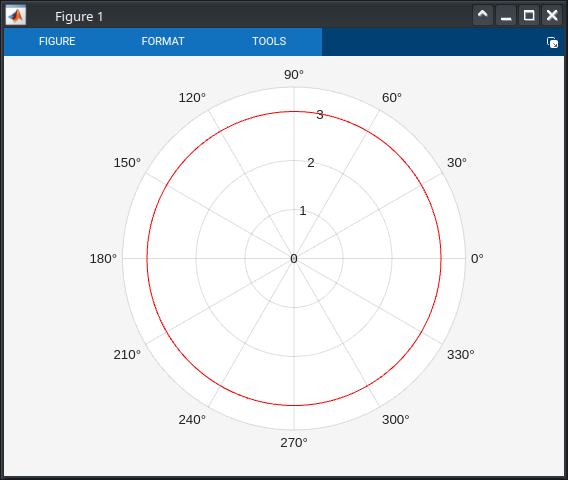
\includegraphics[width=0.6\textwidth]{images/circle.png}
    \caption{example of robot's marginally stable fixed circular motion}
\end{figure}

There are other non-trivial cases too, where certain combinations of initial radial distance \(r_0\) and initial relative heading \(\alpha_0-\theta_0\) for which the robot forever revolves about a point in a fixed circle of radius \(\displaystyle R=\frac{v_0}{K_s}\) not centered at the origin.

The desired relative heading of the robot to head towards home is \(\alpha-\theta=\pi\). Considering this, we can break down the general motion of the robot under given controller into 2 phases:
\begin{enumerate}
	\item An initial phase of circular motion of the robot in a circle of radius \(\frac{v_0}{K_s}\) until its heading is aligned towards the home position, i.e. \(\alpha-\theta=\pi\)
	\item Straight line motion of the robot towards the origin until it reaches home.
\end{enumerate}
The switch from the 1st phase to the 2nd is triggered when its heading aligns towards home. Our hypothesis is that if the robot's initial state and control parameters are such that its heading during the 1st phase never aligns towards the home, it will forever remain stuck in circular motion. This would happen only when one cannot draw a tangent from the origin to the virtual circle of the 1st phase of the robot's motion, which is only possible if the origin lies within said circle. This happens when the distance of the virtual circle's centre from the origin is \(\displaystyle<R=\frac{v_0}{K_s}\).

\begin{figure}[ht!]
	\centering
	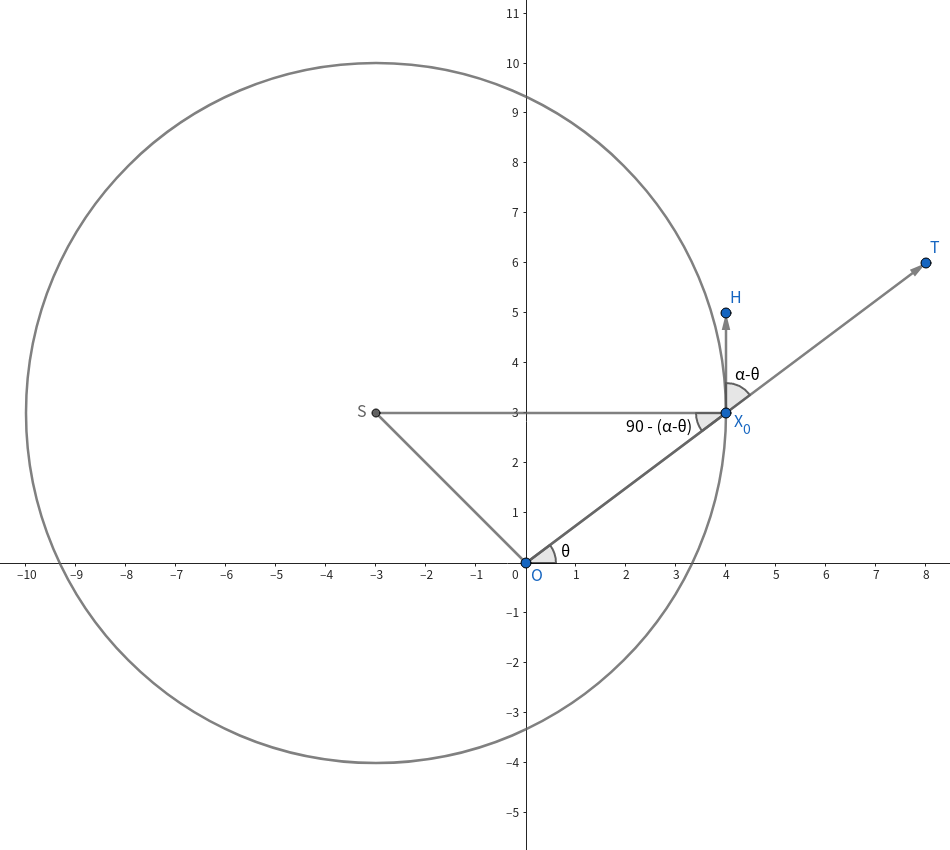
\includegraphics[width=0.75\linewidth]{images/diagram.png}
\end{figure}

Hence, to compute the criteria for marginal stability, one can imagine a triangle \(\Delta OX_0S\) where \(O\) is the home position, \(X_0\equiv(r_0,\theta_0)\) is the initial position of the robot and \(S\) is the centre of the virtual circle.

\(\displaystyle\angle OX_0S=\frac{\pi}{2}-(\alpha-\theta)\) and sides \(\|OX_0\|=r_0\) and \(\displaystyle\|X_0S\|=R=\frac{v_0}{K_s}\). Marginal instability occurs when \(\|OX\|=l<R\). By the cosine law,
\[
	r_0^2 + \cancel{R^2} - 2rR\cos\left(\frac{\pi}{2}-(\alpha_0-\theta_0)\right) < \cancel{R^2}
	\implies r_0^{\cancel{2}} < 2\cancel{r_0}R\sin(\alpha_0-\theta_0)
	\implies \boxed{r_0<2\frac{v_0}{K_s}\sin(\alpha_0-\theta_0)}
\]
Hence, the class of initial conditions satisfying the above inequality will always lead to a marginally unstable response of fixed circular motion.

\end{document}